\section{Sheaf Theory}

Sheaf theory provides a natural mathematical framework for describing how local coherent states combine into global conscious experience. Let $X$ represent the topological space of the brain's cortical sheet, with open sets $U \subseteq X$ corresponding to different cortical regions. A sheaf $\mathcal{F}$ on $X$ assigns to each open set $U$ a collection $\mathcal{F}(U)$ of local sections—mathematical objects that represent coherent energy states within that region.

\begin{figure}[h]
    \centering
    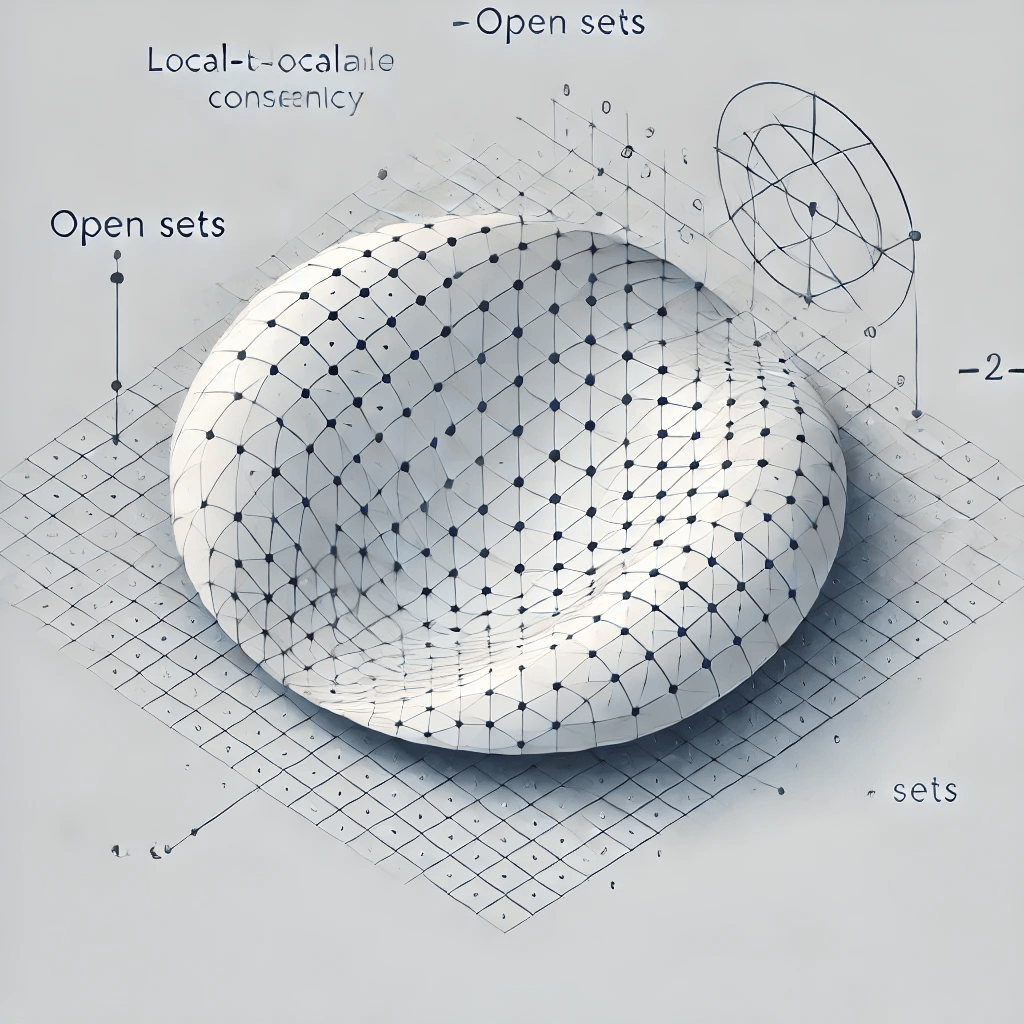
\includegraphics[width=0.8\textwidth]{sheaves.png}

    \caption{Sheaves help us define gluing conditions for consciousness (from local-to-global dynamics)}
\end{figure}

For any two overlapping regions $U$ and $V$, the sheaf includes restriction maps:

\begin{align}
\rho U \cap V: \mathcal{F}(U) \rightarrow \mathcal{F}(U \cap V)
\\
\rho V \cap U: \mathcal{F}(V) \rightarrow \mathcal{F}(U \cap V)
\end{align}


These maps must satisfy the crucial compatibility condition that for any sections $s \in \mathcal{F}(U)$ and $t \in \mathcal{F}(V)$:

$\rho U \cap V(s) = \rho V \cap U(t)$ on $U \cap V$

This compatibility ensures that local coherent states "glue" together properly across regional boundaries. The sheaf structure thus formalizes how consciousness maintains both local specialization and global integration through coherent gluing conditions. These conditions can be expressed through diagrams:

$\mathcal{F}(U) \rightarrow \mathcal{F}(U \cap V) \leftarrow \mathcal{F}(V)$

where the arrows represent restriction maps that must commute for consciousness to maintain coherence.

To capture the rich dynamics of conscious processing, we enhance the basic sheaf structure with additional mathematical machinery. Let $s \in \mathcal{F}(U)$ represent a local section corresponding to a coherent energy state in region U. The section s can be represented as a tuple:

$s = (E, \psi, \phi, \tau)$

where:

- $E$ represents the energy configuration

- $\psi$ captures the electromagnetic field state

- $\phi$ describes chemical gradients

- $\tau$ encodes the transcriptomic profile influencing local dynamics

The global behavior of consciousness emerges from coherent sheaf dynamics, where multiple local sections must satisfy compatibility conditions across overlapping regions. For regions $U$, $V$, $W$ with non-empty intersections, we require:

1. Binary Compatibility:
$\rho_{U \cap V}(s_U) = \rho_{V \cap U}(s_V) \text{ on } U \cap V$

2. Triple Overlap Condition:
$\rho_{U \cap V \cap W}(s_U) = \rho_{V \cap W \cap U}(s_V) = \rho_{W \cap U \cap V}(s_W) \text{ on } U \cap V \cap W$

These conditions ensure hierarchical coherence stability. The framework introduces a coherence measure $\mu$ that quantifies the degree of alignment between local sections:

$\mu(s_U, s_V) = \int_{U \cap V} \|\rho_{U \cap V}(s_U) - \rho_{V \cap U}(s_V)\|^2 \,d\nu$

where $d\nu$ represents an appropriate measure on the overlap region. Conscious processing requires that $\mu$ remains below certain thresholds determined by the brain's energetic constraints.

The global section of consciousness, $S \in \mathcal{F}(X)$, must satisfy not only local coherence conditions but also maintain stability under coherent deformation operators $D\lambda$:

$D\lambda(S)|_U = s_U + \delta\lambda(s_U)$

where $\delta\lambda$ represents small perturbations that model the continuous adaptation of conscious states. The existence of stable global sections requires that:

$\sup\{\mu(D\lambda(S)|_U, D\lambda(S)|_V)\} < \varepsilon$

for some small $\varepsilon > 0$ across all overlapping regions $U$, $V$ and allowable deformations $\lambda$.

This sheaf-theoretic framework naturally extends to incorporate the dynamics of energy flows through a coherent energy complex, leading us to consider the stress-energy tensor formalism in the next section.

For readers interested in deepening their understanding of sheaf theory and its applications to consciousness and computation, several key texts provide valuable foundations. The classic introduction \cite{MacLane1992} offers a comprehensive treatment of sheaves in both geometric and logical contexts, particularly useful for understanding the mathematical underpinnings of local-to-global transitions. For those seeking a more modern treatment, \cite{Kashiwara2005} presents advanced perspectives on categories and sheaves that illuminate the formal structures underlying coherent integration. The application of sheaf theory to concurrent and interactive systems, as detailed in \cite{Goguen1992}, provides crucial insights into how sheaf-theoretic approaches can model complex, distributed processes. Of particular relevance to consciousness studies is \cite{Rushworth2018}, which develops a categorical framework for consciousness using sheaf theory, demonstrating how these mathematical tools can bridge local neural dynamics and global conscious states. For those interested in the broader philosophical implications, \cite{Rosen1991} explores how sheaf-theoretic concepts illuminate fundamental questions about biological organization and cognition. These works collectively demonstrate how sheaf theory provides a rigorous mathematical framework for understanding the emergence of unified conscious experience from distributed neural processes.